\documentclass[10pt]{article}
\usepackage[margin=0.75in]{geometry}
\usepackage{amsmath,amssymb,booktabs,enumitem,url,hyperref,graphicx}
\hypersetup{hidelinks}
\title{Supplementary Material for\\Verifiable Matrix Maintenance with Fresh Work Guarantees}
\author{Chuanliu Liu \and Zhirong Yue \and Rong Du \and Yue Fu \and Yongle Chen\\
Taiyuan University of Technology}
\date{}
\begin{document}
\maketitle

This document records details that are intentionally kept out of the twelve-page
main paper: the complete experimental protocol, the variance calculation for
the randomized views, additional certificate diagnostics, and a file-level
reproduction map. It is distributed with the public artifact at
\href{https://github.com/fuyuefyu/verifiable-matrix-maintenance}{the project repository}.

\section{Protocol and frozen study units}
The matrix-engine study has a 73-cell parameter grid and six long-stream
runs, for 176,520 method--round records. Every cell has five workload seeds
and three repeats. Per-update estimates take the median over rounds, repeats,
and then seeds; speedups are paired within seed. The nominal 95\% intervals
are percentile-bootstrap intervals from 2,000 resamples of the five seed
summaries. Cumulative bands are pointwise and include initialization.

The Covertype extension fixes $b=8$, $t=2$, and $k=256$. It runs
$n\in\{256,512,1024\}$ on server GPU2, $n\in\{512,1024\}$ on a Spark
CPU, and one synchronized $n=1024$ diagnostic. Jobs are sequential within
each host. The connected study has twenty same-tape $q=17$ replay pairs,
twenty fresh source-paired streams per encoding for $q=65521$, and twenty
independent utility simulations. Replaying a tape is not counted as a new
fresh-work episode.

The artifact records source identities, seeds, setup costs, and timing
boundaries. Dense GPU experiments use $q=65521$, $n=4096$, $r=8$, and
$t=2$; the structured view uses 54 features over the same field with
$n=1024$, $b=8$, and $t=2$. The connected service comparison uses the Spark-
ebaf CPU and fy RTX 5090 GPU0. These labels identify the measured hosts; they
are not claims about pooled populations.

\section{Randomized-view variance calculation}
Let $H$ be the true $n\times n$ count table and let the released estimate be
$\widehat H$. The report mechanisms are symmetric unary encoding (SUE) and
optimized unary encoding (OUE), both members of the randomized-response family
used in the main paper \cite{warner1965randomized,erlingsson2014rappor,dworkroth2014}.
We use the frequency MSE
\[
  \mathrm{MSE}=n^{-2}\lVert \widehat H/N-H/N\rVert_F^2.
\]
For a single attribute, write
\[
 \sigma_0^2=\frac{\beta(1-\beta)}{(p-\beta)^2},\qquad
 \sigma_1^2=\frac{p(1-p)}{(p-\beta)^2}.
\]
Independence of attribute noises gives the per-record sum of cell variances
\[
 \bigl[(n-1)\sigma_0^2+\sigma_1^2+1\bigr]^2-1.
\]
For the equal-parameter strata used in the plots, this yields
\[
 \mathbb E[\mathrm{MSE}]_{\mathrm{SUE}}=\frac{47}{20N},\qquad
 \mathbb E[\mathrm{MSE}]_{\mathrm{OUE}}=
 \frac{1925689}{1036800N}.
\]
The plotted reference is the square root of these expressions. Across four
nested prefixes and both encodings, empirical means are within 0.8\% of the
corresponding analytical values. At $N=581{,}012$, the root MSEs are
$2.018\times10^{-3}$ (SUE) and $1.781\times10^{-3}$ (OUE), with paired
ratio $1.133$ and nominal interval $[1.123,1.142]$.

\section{Checking certificates and allocation}
For the $q=17$ study, the target is
$\delta=(31/50)^{64}=5.165\times10^{-14}$. The exact heterogeneous
allocator (OPT) certifies 767 checks. Certificate-marginal greedy reaches the same
schedule; fixed-prefix round robin (RR) requires 856 checks. The budgets 766 and
855 fail their exact target tests. The allocator agrees with exhaustive
enumeration on 162 small cases (6,804 allocations) and 56 full-size
comparisons. Complete plan generation costs are 3.473 ms (OPT) and 2.743 ms
(RR). A separate search-only comparison gives medians 1.553, 0.866, and
34.443 ms for OPT, RR, and certificate-marginal greedy, respectively; those
times exclude serialization and output validation.

For the fresh-input service, the common integrity budget is
\[
 I(\mathbf t)\le \varepsilon=512/q^2=1.193\times10^{-7},
 \qquad q=65521.
\]
Because one check already exceeds this budget, every round uses at least two
checks and $T\ge1024$. Uniform $t=2$ attains this minimum for both policies.
SUE meets the stated work target with bound $1.893\times10^{-14}$; OUE's
threshold floor $4.105\times10^{-4}$ rules out that target. These are
analytical certificates, not measured attack probabilities.

\section{Additional timing diagnostics}
The complete-update GPU comparison at $n=4096$, $r=8$, and $t=2$ is
83.162 ms for checked maintenance versus 161.931 ms for checked
recomputation. The width sweep reaches 1.968$\times$ at $r=32$; at
$n=1024$, the speedup decreases from 1.256$\times$ at $r=2$ to
0.997$\times$ at $r=512$. The checking factors for $t=1,2,4,8$ are
1.130, 1.101, 1.099, and 1.111.

For the structured view, full product construction is 1.483 ms, the generic
increment is 0.0702 ms, and the cached increment is 0.0588 ms. Candidate
freezing and checking are 3.032 ms and 0.441 ms for the generic path.
Setup-inclusive medians over 256 updates are 1750.736, 1330.161, and
1325.996 ms for recomputation, generic maintenance, and cached
factorization. At $n=256$ and $512$, GPU speedups are 0.932 and 0.982;
the corresponding intervals include parity.

The CPU extension at $n=1024$ takes 10.234 ms versus 21.468 ms,
giving 2.098$\times$ with interval $[2.086,2.112]$. Its setup-inclusive
totals are 2645.888 and 5520.294 ms; caching adds 1.020$\times$ with
interval $[1.010,1.029]$. Across four GB10 devices, dense speedups range
from 1.225$\times$ to 1.925$\times$; devices are therefore not pooled.

\section{Full Covertype view diagnostics}
Figures~\ref{fig:application-results} and~\ref{fig:view-costs} retain the
individual utility, accuracy, and checking-cost units summarized in the main paper.
% Generated application_results.pdf is copied into manuscript/figures/.
% This caption specifies the estimands without presupposing a favorable outcome.
\begin{figure*}[t]
  \centering
  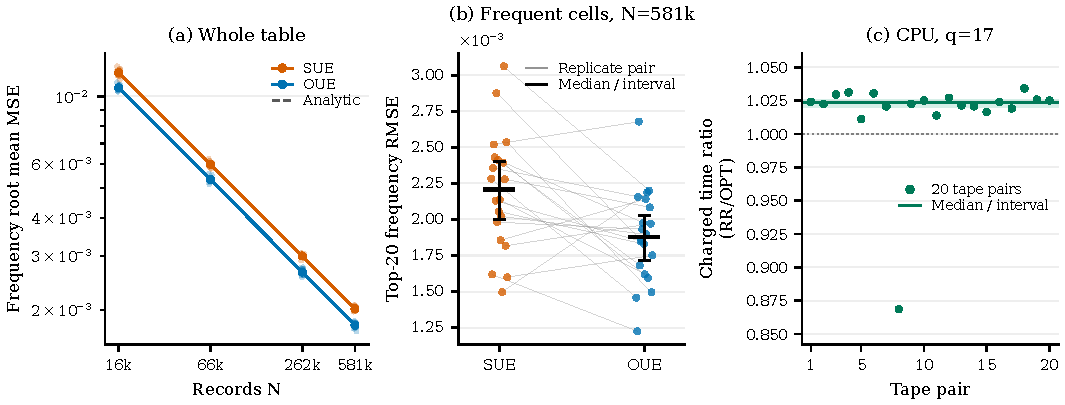
\includegraphics[width=\textwidth]{figures/application_results.pdf}
  \caption{Covertype randomized-view accuracy and checking-cost diagnostics for SUE and OUE over nested prefixes and paired streams.}
  \label{fig:application-results}
\end{figure*}

\begin{figure*}[t]
  \centering
  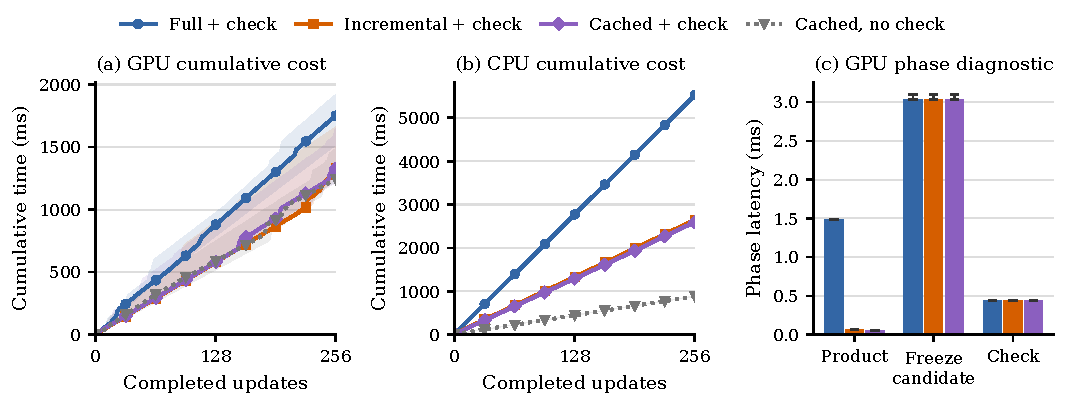
\includegraphics[width=\textwidth]{figures/view_costs.pdf}
  \caption{Covertype row-replacement cumulative and phase costs for recomputation, incremental maintenance, and cached factorization over $\mathbb{F}_{65521}$.}
  \label{fig:view-costs}
\end{figure*}


\section{Reproduction map}
The public repository contains the frozen source files, lightweight inputs,
plans, and code used for the reported measurements. From a Linux environment
with Python 3.10 or newer, a configuration-only check is:
\begin{verbatim}
python reproduce.py --profile planner \
  --deadline-utc 2030-01-01T00:00:00Z \
  --max-seconds 900 --out reruns/planner-dry --dry-run
\end{verbatim}
The bounded process-group controller is Linux-only and does not download
packages, credentials, or datasets. Connected and GPU profiles require the
corresponding local hardware and an explicit future deadline. The manifest
records source hashes and the derived command; a dry run is a configuration
check and does not claim a new scientific execution.

\bibliographystyle{IEEEtran}
\bibliography{references}
\end{document}
